273. В углу прямоугольника $3\times6$ стоит кубик (размер грани кубика совпадает с клеткой). У данного кубика сильно испачкана одна грань. Можно перекатывать кубик через ребро, при этом запрещено выкатывать его за пределы прямоугольника и ставить на клетку, на которой кубик уже стоял. Придумайте способ испачкать как можно больше клеток прямоугольника. Какая именно грань кубика запачкана, вы можете выбрать сами. В каждой клетке прямоугольника запишите, какой по счёту эта клетка окажется под кубиком (в клетке, на которой кубик стоит изначально, запишите число 1). В ответ запишите число испачканных клеток.
\begin{center}
\begin{figure}[ht!]
\center{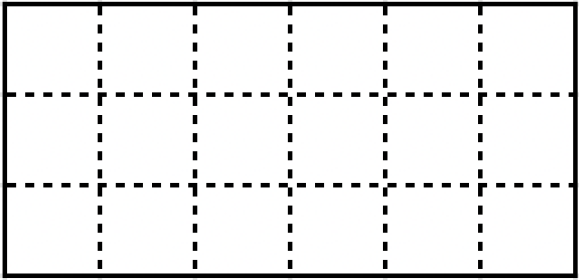
\includegraphics[scale=0.35]{kub2.png}}
\end{figure}
\end{center}
